% EMNLP 2026 -- System Demonstrations Track
% Main paper file for Overleaf / ACL style compilation.

\documentclass[11pt]{article}

% Use ACL style. For final camera-ready, remove [preprint] if required by the venue.
\usepackage[preprint]{acl}

% Standard packages.
\usepackage{times}
\usepackage{latexsym}
\usepackage{graphicx}
\usepackage{url}
\usepackage{amsmath}
\usepackage{microtype}
\usepackage{xcolor}
\usepackage{array}

% ACL template setting.
\renewcommand{\UrlFont}{\ttfamily\small}

% Single-blind demo review allows author names to remain visible.
% Keep the simple ACL/EMNLP author-block style.
\title{LuxLLM-Agent: An Inspectable LLM-Assisted Agent and Replay Viewer for Lux AI Season 3}

\author{
  First Author \\
  Affiliation / Address line 1 \\
  Affiliation / Address line 2 \\
  Affiliation / Address line 3 \\
  \texttt{email@domain} \\
  \And
  Second Author \\
  Affiliation / Address line 1 \\
  Affiliation / Address line 2 \\
  Affiliation / Address line 3 \\
  \texttt{email@domain}
}

\begin{document}
\maketitle

\begin{abstract}
We present LuxLLM-Agent, an inspectable LLM-assisted agent system for Lux AI Season 3. The system combines a local game-playing agent, rule-based fallback policies, structured decision logs, and an isometric battle replay viewer for analysing agent behaviour. Unlike a standard replay viewer, our interface connects game states with decision traces, cached LLM decisions, fallback events, match-level scores, and final result summaries. We evaluate the system through controlled \texttt{qwen3:32b} matches on Barkla2, where a target-aware strategic planner improves the LLM-assisted player's descriptive win rate from 56\% to 70\% over a previous basic qwen3 planner while maintaining zero LLM errors. The system also includes a lightweight scalability simulation with up to 1000 worker agents. The demo package includes a replay viewer, screenshots, replay JSON, evaluation reports, and screencast material for research and educational use.
\end{abstract}

\section{Introduction}

Large language models (LLMs) have become increasingly attractive for building agents that can reason over complex environments, generate high-level plans, and expose intermediate reasoning traces. However, game-agent settings expose several practical challenges that are easy to overlook in isolated prompting examples. The environment is dynamic, action legality matters, repeated model calls are expensive, and final match outcomes alone do not explain why an agent behaved in a particular way. These challenges are especially visible in long-horizon games where performance emerges from many small tactical decisions rather than from a single model response.

This paper presents LuxLLM-Agent, a system demonstration focused on making LLM-assisted game agents inspectable and reproducible. The system targets Lux AI Season 3~\citep{luxai2024}, a competitive two-player game environment involving exploration, hidden map information, unit movement, scoring opportunities, energy-related constraints, and long-horizon tactical decisions. Rather than presenting the agent as a competition-winning policy, we use the environment as a compact testbed for studying how LLM-generated strategies can be connected to fallback-safe execution and replay-grounded analysis.

The central idea is to treat the LLM as a high-level strategy component rather than as a direct controller for every individual unit action. The agent records structured decision traces, reuses cached strategy decisions between fresh LLM calls, and falls back to deterministic rules when the LLM is unavailable, too slow, or unsuitable for direct execution. The replay viewer then makes these decisions visible alongside the game state, helping users inspect how the agent combines LLM strategy, cached decisions, rule fallback, and match outcomes.

This setting raises a different research question from simply maximising leaderboard performance: how can an LLM-assisted game agent be made observable enough for users to inspect its decisions after a match? In many agent demonstrations, the LLM component is only visible through a final action or through a natural-language explanation generated after the fact. LuxLLM-Agent instead records decision-source metadata during execution and binds these records to replay frames. This makes it possible to distinguish between fresh LLM decisions, cached LLM decisions, deterministic fallback actions, and rule-controlled opponent actions.

The contribution of this demo is system-oriented. First, it provides a fallback-safe LLM-agent runtime for Lux AI Season 3, where high-level LLM strategy generation is separated from low-level action validation. Second, it introduces replay-grounded decision traceability, allowing users to inspect how decisions were produced during the match rather than relying only on final scores. Third, it reports controlled \texttt{qwen3:32b} evaluation results together with trace coverage, fallback behaviour, latency, and cached-decision statistics. Finally, it includes a lightweight scalability simulation showing how sparse LLM-generated policy templates can be reused by many cheaper worker agents.

\section{System Overview}

LuxLLM-Agent consists of a local Lux AI Season 3 agent, an LLM-assisted decision layer, a fallback-safe execution layer, a trace logger, an evaluator, and a replay-grounded viewer. Figure~\ref{fig:replay-viewer} shows the replay interface used in the demonstration.

\begin{figure}[t]
\centering
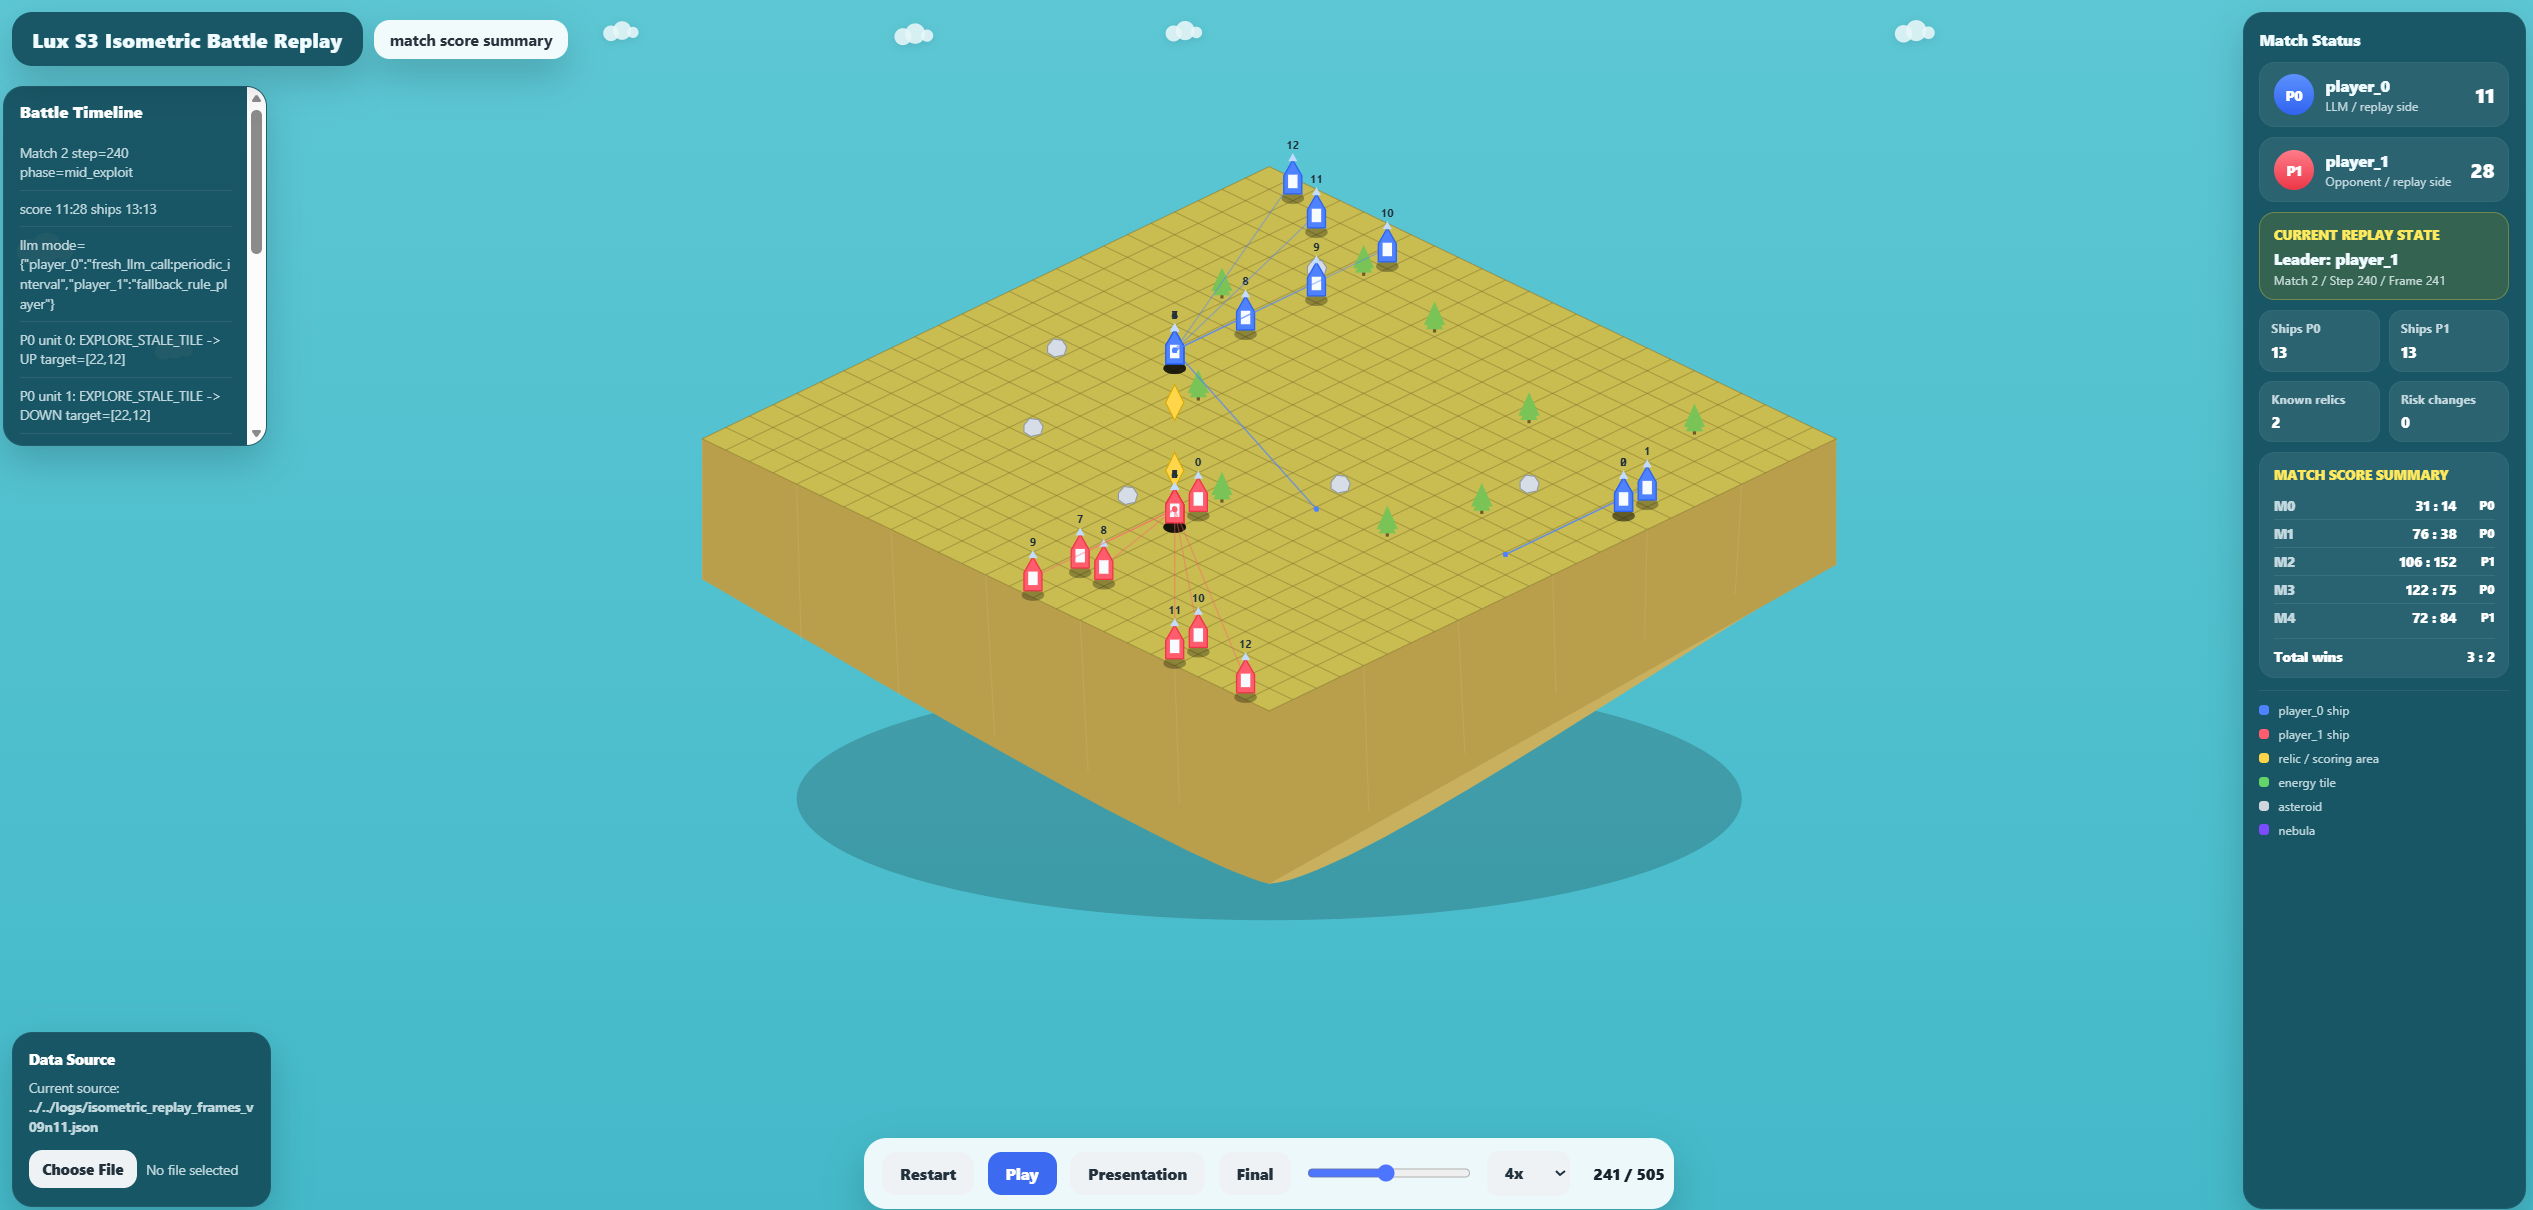
\includegraphics[width=\linewidth]{figures/figure_s3_replay_viewer.png}
\caption{Replay viewer for inspecting Lux AI Season 3 matches. The viewer shows the game map, unit positions, score progression, final result information, and decision-related metadata.}
\label{fig:replay-viewer}
\end{figure}

\subsection{Runtime Components}

The system separates strategy generation, safe execution, trace logging, replay inspection, and evaluation. The agent runtime executes Lux AI Season 3 matches and converts validated decisions into game actions. The LLM layer generates sparse high-level strategies from compact state summaries. A cache layer reuses previous LLM decisions across turns to reduce repeated model calls. A deterministic fallback policy maintains safe execution when the LLM is unavailable, too slow, or unsuitable for direct execution. A trace logger records frame-level decision provenance and match metadata, while the evaluator produces match summaries, controlled metrics, and evidence reports. Finally, the replay viewer visualises match state, score progression, and decision evidence.

This component separation is important for inspectable LLM-agent systems. If the LLM, action executor, logger, and viewer are tightly coupled, it becomes difficult to identify whether an observed behaviour came from model reasoning, cached strategy reuse, deterministic rules, or replay post-processing. LuxLLM-Agent therefore treats the agent runtime and the replay viewer as connected but separate components: the runtime produces structured evidence, and the viewer renders that evidence for inspection.

\subsection{Agent Runtime}

The game-playing agent runs inside the Lux AI Season 3 environment. At each decision point, the runtime extracts compact state features from the current observation, including unit locations, visible map information, energy-related signals, known scoring opportunities, and recent match context. These features are converted into a compact decision summary for the LLM-assisted layer.

The system does not ask the LLM to directly output arbitrary low-level commands for every unit. Instead, the LLM produces structured strategic decisions, such as whether to explore, move towards candidate scoring tiles, preserve units, or follow a previously selected plan. Low-level action conversion remains rule-checked so that the executed actions stay compatible with the environment.

\subsection{Data Flow and Decision Sources}

The system follows a frame-level data flow. For each game frame, the runtime receives an observation from the Lux AI environment and extracts a compact state representation. This representation includes visible unit positions, local map evidence, known or suspected scoring opportunities, energy-related information, and recent strategy context. The summarised state is then passed either to the LLM-assisted strategy layer or to the deterministic fallback layer, depending on the current decision schedule and runtime conditions.

Each executed action is annotated with a decision source. We use four decision-source categories. A \emph{fresh LLM decision} indicates that the current action was derived from a newly generated model response. A \emph{cached LLM decision} indicates that the agent reused a previously generated strategy without making a new model call. A \emph{fallback decision} indicates that the system used deterministic rules because the LLM was unavailable, too slow, or unsuitable for direct execution. A \emph{rule-player decision} corresponds to the non-LLM baseline opponent in controlled evaluation. These categories are stored in the replay trace so that decision provenance can be inspected after the match.

This separation is important because LLM-based agents can otherwise be difficult to evaluate. A match outcome alone does not show whether the LLM contributed useful strategic information, whether the system relied mostly on fallback rules, or whether the agent repeatedly reused an old decision. By recording decision sources at runtime, LuxLLM-Agent exposes the operational structure of the agent and supports more precise analysis than final win rate alone.

\subsection{LLM-Assisted Strategy Layer}

The current controlled experiments use a local Ollama backend~\citep{ollama2024} with \texttt{qwen3:32b}~\citep{yang2025qwen3} served on Barkla2 GPU resources. The LLM is queried sparsely rather than on every frame. Fresh LLM decisions are recorded as structured JSON-like decisions, while cached LLM decisions are reused across later turns when appropriate. This design reduces repeated model calls and makes it possible to compare fresh model decisions, cached decisions, and fallback events in the same replay trace.

The strategy layer is deliberately constrained. It receives a compact state summary rather than the full raw game state, and it returns a bounded decision object rather than free-form executable code. This reduces parsing ambiguity and allows the downstream runtime to validate decisions before execution. The design also makes the decision trace easier to inspect because the output categories are stable across matches.

The system records LLM latency, parsing results, decision source, selected strategy, and fallback status. These logs are used both for quantitative evaluation and for visual inspection in the replay viewer.

\subsection{Fallback-Safe Execution}

The runtime includes deterministic fallback policies that are used when the LLM call times out, returns unusable content, or when rule-level action safety is required. The fallback policy also controls the non-LLM opponent in the controlled evaluation. This fallback design is important for long-horizon game-agent demos because a single failed model call should not terminate the whole match or invalidate the replay.

Fallback is not treated as a failure of the system. Instead, it is part of the execution architecture. In a practical LLM-agent runtime, model latency, parsing errors, and environment constraints are expected operational conditions. The goal is therefore not to remove all fallback behaviour, but to make fallback explicit, measurable, and inspectable.

\subsection{Replay-Grounded Viewer}

The replay viewer links match frames with decision traces. Users can inspect not only the final score but also which decision source was active at a given stage: fresh LLM decision, cached LLM decision, rule fallback, or rule-controlled opponent action. This makes the system more useful as a teaching and research demo than a simple final-score replay.

The viewer is designed around replay-grounded decision traceability. It does not claim to provide a complete causal explanation for every action. Instead, it exposes recorded evidence: the state summary used by the system, the selected decision source, the cached or fresh strategy status, fallback indicators, and match-level outcome summaries. This gives users a concrete basis for analysing agent behaviour.

\section{Demonstration Walkthrough}

The demo begins with a completed Lux AI Season 3 match replay. The user opens the local HTML viewer and sees the map, units, score progression, final result overlay, and decision-related panels. The viewer can be used in a live demo or recorded screencast.

The first part of the walkthrough introduces the match-level view: the current turn, both players' scores, unit locations, visible tiles, and final result summary. This allows users to understand the game context before inspecting the agent's decisions.

The second part focuses on the decision trace. The presenter shows how the viewer distinguishes between fresh LLM decisions, cached LLM decisions, fallback actions, and rule-player actions. This is the key difference between LuxLLM-Agent and a normal replay viewer: the system connects what happened in the match with why the agent selected a strategy at that moment.

The third part demonstrates evaluation artefacts. The system produces Markdown summaries, JSON evaluation files, structured logs, replay frames, and screenshots. These artefacts allow a user to reproduce the paper's reported results, inspect a specific match, or compare design variants.

During the live demonstration, the presenter can pause on selected replay frames and explain the associated decision source. For example, a frame may show that the agent is following a cached strategy rather than querying the LLM again, or that a fallback rule was used to preserve execution safety. The viewer also supports comparison between local map evidence and match-level outcome summaries. This interaction is useful for debugging because it allows users to identify whether a poor outcome was caused by strategic selection, stale cached decisions, fallback behaviour, or local movement constraints.

The intended takeaway is not that every individual action is accompanied by a perfect natural-language explanation. Instead, the demo shows a practical inspection workflow for LLM-assisted agents: run a controlled match, collect structured traces, replay the match, inspect decision provenance, and compare summary metrics across configurations. This workflow is especially relevant for game-agent research because long-horizon behaviour often emerges from many small decisions rather than from a single model output.

Figure~\ref{fig:presentation-mode} shows the presentation-oriented interface used for demonstration recording.

\begin{figure}[t]
\centering
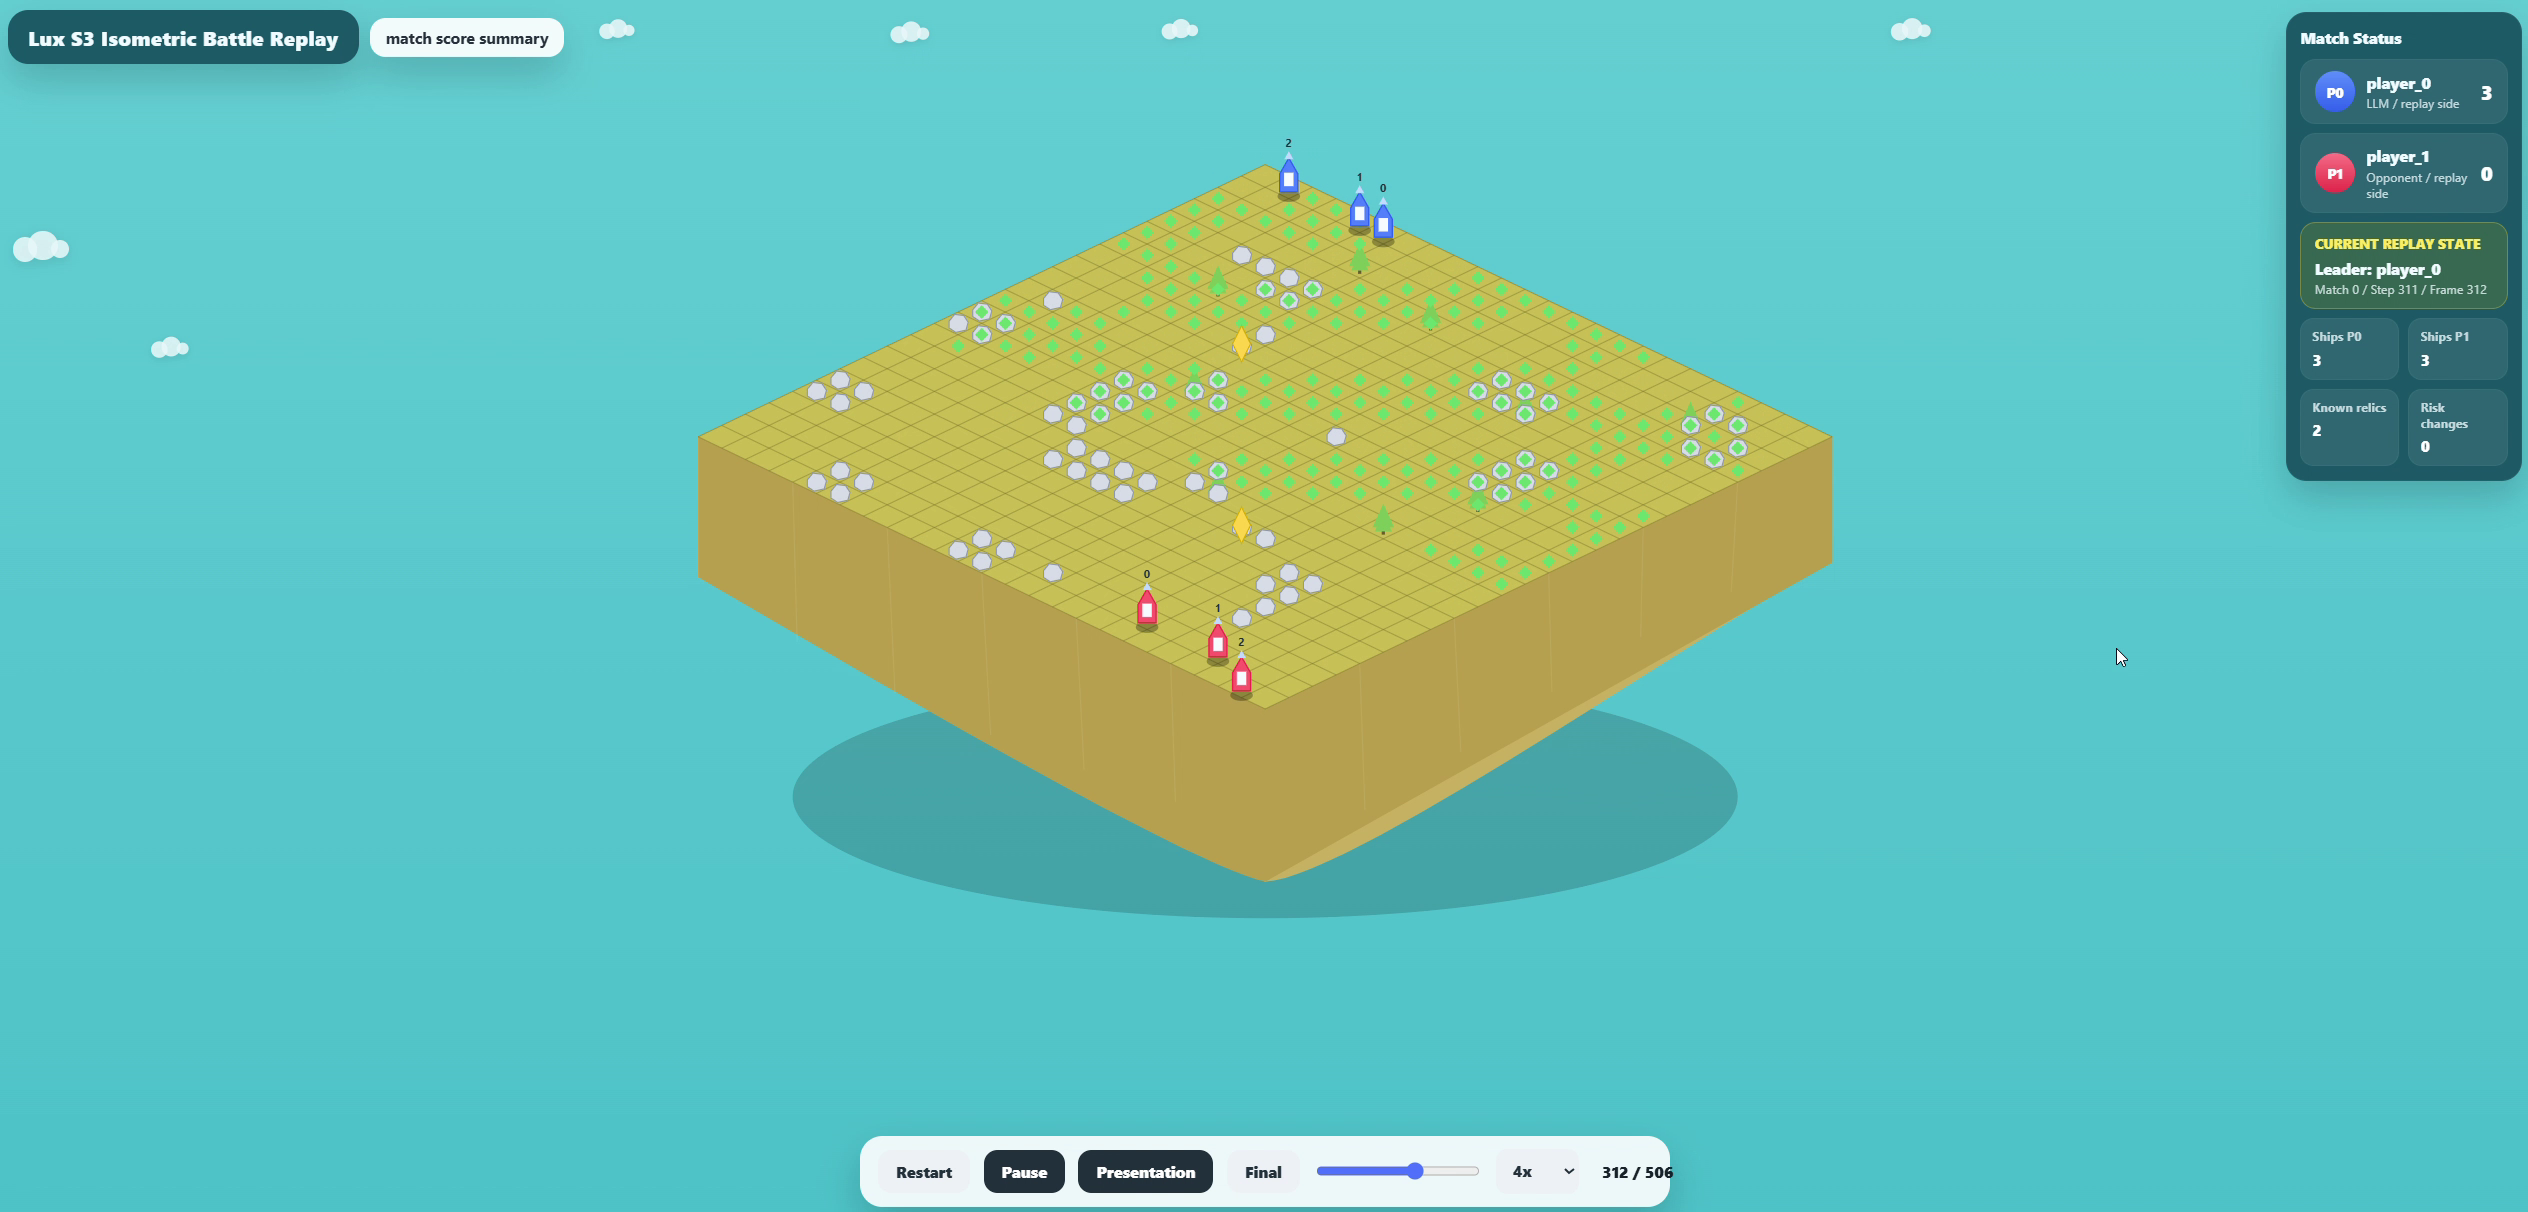
\includegraphics[width=\linewidth]{figures/figure_s3_presentation_mode.png}
\caption{Presentation-oriented replay view. The interface is designed to show both game progress and decision evidence during a short demo video.}
\label{fig:presentation-mode}
\end{figure}

\section{Implementation}

The prototype is implemented in Python and JavaScript. The Lux AI Season 3 agent runs locally through the competition environment, while LLM inference is served by a local Ollama backend. Controlled experiments use \texttt{qwen3:32b} on Barkla2 GPU resources. The implementation records console logs, structured JSONL frame logs, LLM decision traces, evaluation JSON files, replay frames, screenshots, and Markdown summaries.

The viewer is implemented as a standalone HTML interface that can be opened through a local HTTP server. It is intended for both live demonstration and video recording. The system keeps the replay artefacts separate from the agent runtime so that recorded matches can be inspected after execution without rerunning the game.

The implementation follows three design principles. First, LLM decisions should be structured enough to analyse automatically. Second, rule fallback should keep the game executable even when model calls fail or become too slow. Third, replay artefacts should remain human-readable so that students and researchers can inspect the agent without needing to understand every implementation detail.

The runtime also separates evidence generation from presentation. Match execution produces raw logs and JSONL traces, while post-processing scripts summarise these traces into evaluation reports and viewer-ready replay data. This separation is useful because the same match can be inspected at multiple levels: raw console output for debugging, structured traces for quantitative analysis, and the visual replay for demonstration.

\section{Evaluation}

We evaluate LuxLLM-Agent from three perspectives: controlled match outcome, replay-grounded decision traceability, and architecture-level scalability. The purpose of this evaluation is not to claim state-of-the-art Lux AI performance, but to validate the stability and inspectability of the proposed LLM-assisted agent pipeline. We therefore report match outcomes together with decision-source statistics, fallback behaviour, cached-decision reuse, LLM latency, and trace coverage.

\subsection{Controlled Match Evaluation}

All controlled matches use the same local agent interface, the same replay logging pipeline, and the same post-processing scripts. The LLM-assisted player is evaluated against a deterministic rule-controlled opponent. This design does not aim to benchmark against the full Lux AI competition leaderboard; instead, it isolates whether the LLM-assisted runtime can execute complete matches, produce inspectable traces, and remain stable across repeated runs. We report win counts as a coarse behavioural outcome, while trace coverage, LLM error count, latency, fallback count, and decision-source statistics are used to evaluate system reliability.

The win count measures how often the LLM-assisted player obtains the better final match result under the controlled setting. The LLM error count measures failed or unusable model interactions after parsing and runtime checks. Trace steps measure how many frame-level records are available for replay-grounded inspection. Fresh LLM decisions count newly generated model responses, while cached LLM decisions count turns where the system reuses a previous strategy. These metrics are important for a system demonstration because they show whether the agent is merely producing occasional successful matches or whether it consistently generates complete, inspectable execution records.

The previous basic \texttt{qwen3:32b} planner uses compact structured JSON decisions and deterministic fallback. In a 50-match controlled evaluation, the LLM-assisted player won 28 matches against 22 wins for the rule-controlled opponent. This run achieved a strategy-use rate of 92.7\%, a fallback rate of 7.3\%, and zero LLM errors.

The current target-aware \texttt{qwen3:32b} strategic planner extends the basic interface with target coordinates, priority scores, risk labels, expected-value estimates, and lightweight rule-based arbitration. In a separate 50-match controlled evaluation, the LLM-assisted player won 35 matches against 15 wins for the rule-controlled opponent. This corresponds to a descriptive win rate of 70\%, with a strategy-use rate of 96.0\%, a fallback rate of 4.0\%, and zero LLM errors.

Earlier strategy-diverse prompting and candidate-exploitation configurations are retained as development evidence and ablation context. They show that the same evaluation pipeline can compare design variants, but they are no longer treated as the final main result.

\begin{table*}[t]
\centering
\small
\begin{tabular}{lcccccc}
\hline
Configuration & Runs & LLM wins & Rule wins & Win rate & Strategy use & Fallback \\
\hline
Basic qwen3 planner & 50 & 28 & 22 & 56\% & 92.7\% & 7.3\% \\
Target-aware qwen3 strategic planner & 50 & 35 & 15 & 70\% & 96.0\% & 4.0\% \\
Strategy-diverse prompting & 50 & 29 & 21 & 58\% & -- & -- \\
Candidate-exploitation ablation & 50 & 26 & 24 & 52\% & -- & -- \\
\hline
\end{tabular}
\caption{Controlled \texttt{qwen3:32b} evaluation on Barkla2. The target-aware strategic planner is the current main controlled result, while earlier prompting variants are retained as development evidence and ablation context. All reported qwen3 runs completed with zero LLM errors.}
\label{tab:qwen3-controlled-eval}
\end{table*}

For the current target-aware strategic planner, the decision logs contain 1249 fresh LLM calls, 1199 strategy-used decisions, and 50 fallback events across the 50-match run. These statistics show that the system is not merely calling an LLM once for a static plan. Instead, it combines structured LLM planning, schema validation, rule-based arbitration, and fallback-safe execution.

The results should be interpreted as evidence of controlled runtime stability and inspectability rather than as proof of optimal game-playing strength. The target-aware strategic planner achieved the strongest 50-match controlled result in the current project state, while earlier prompting variants remain useful for understanding the design space.

Figure~\ref{fig:score-summary} summarises match-level score and result information from the replay artefacts.

\begin{figure}[t]
\centering
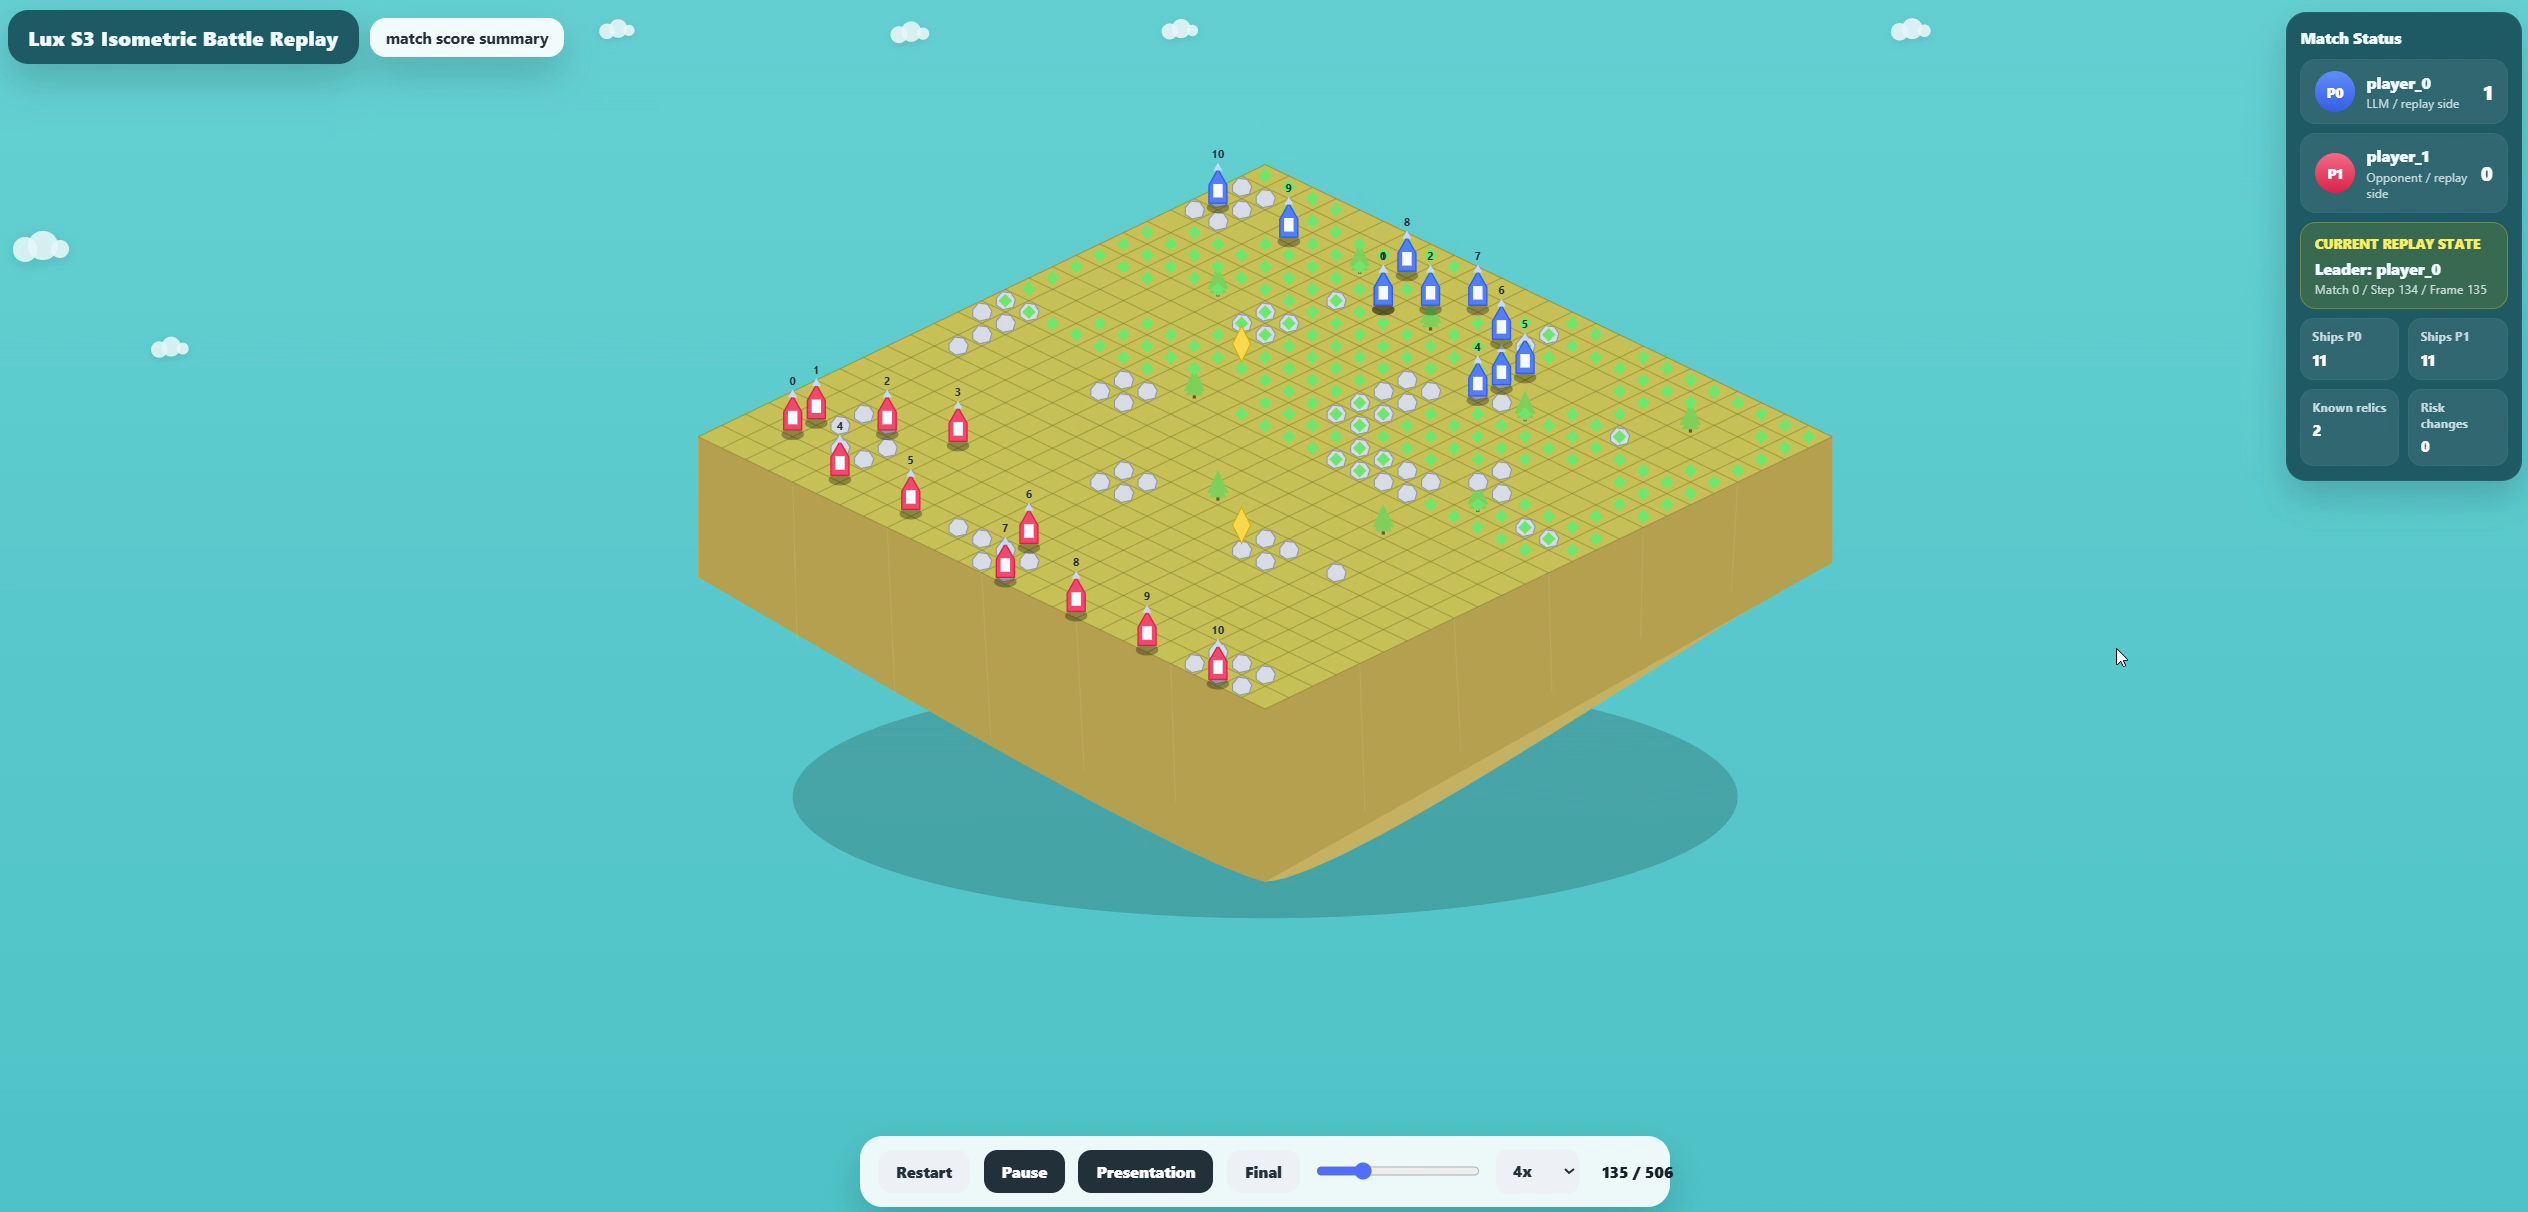
\includegraphics[width=\linewidth]{figures/figure_s3_match_score_summary.png}
\caption{Match score summary produced from replay and evaluation artefacts. The demo connects final results with decision traces rather than presenting only the final score.}
\label{fig:score-summary}
\end{figure}

\subsection{Replay-Grounded Decision Traceability}

The replay viewer provides qualitative evidence that the decision trace can be inspected after a match has completed. Each replay frame can be connected to decision-source metadata, including fresh LLM decisions, cached LLM decisions, fallback actions, and rule-player actions. This supports debugging and teaching because users can follow how a high-level decision is reused across multiple turns and how fallback prevents failed model calls from breaking match execution.

This evaluation does not claim that the viewer fully explains all causes of agent behaviour. Instead, it provides replay-grounded decision traceability: the user can inspect recorded decision sources, selected strategies, fallback status, and match outcomes in a single interface.

The viewer also makes stale or reused decisions visible. This is important because cached LLM strategies can be beneficial when they reduce latency and preserve consistent behaviour, but they can also become harmful if the local environment changes faster than the strategy is refreshed. By logging cached decision reuse explicitly, the system allows users to diagnose whether an observed behaviour came from a fresh model response, a reused strategy, or a fallback rule.

\subsection{Scalability Simulation}

The system also includes a lightweight scalability simulation. This simulation does not run 1000 full Lux AI game instances. Instead, it tests whether sparse LLM-generated policy templates can be reused across many lightweight worker agents. The simulation verifies that the architecture can separate expensive strategy generation from cheaper worker-level execution. The result supports the architectural claim that sparse LLM calls and cached policy reuse can scale better than direct per-agent LLM control.

The scalability result should therefore be interpreted as architecture-level evidence rather than as a direct measurement of competitive multi-agent performance. Its purpose is to test whether the system design can support many worker-level decisions once a small number of LLM-generated policies are available. This complements the controlled match evaluation by examining a different system property: reuse of expensive model-generated strategy under lightweight execution.

\section{Comparison with Existing Systems}

Most game replays focus on visualising what happened during a match. They show map states, unit movements, and final scores, but they usually do not connect these events to the decision process of an LLM-assisted agent. LuxLLM-Agent focuses on the connection between match replay and decision evidence.

Compared with direct LLM control, our system uses the LLM as a sparse strategic component and keeps low-level execution guarded by deterministic rules. Compared with a pure rule-based baseline, the system records structured LLM decisions and cached strategy reuse, allowing users to inspect where the LLM influenced the agent. Compared with generic agent frameworks, the system is grounded in a reproducible game environment with replay artefacts and controlled match evaluation.

The system is also different from post-hoc explanation interfaces. A post-hoc explanation can describe an action after the match, but it may not correspond to the actual runtime mechanism that produced the action. LuxLLM-Agent instead records decision-source information during execution and displays it through the replay artefact. This makes the inspection process more directly connected to the executed system.

\section{Licensing and Availability}

The demo package is intended to be released with source code, replay artefacts, screenshots, evaluation summaries, and screencast material. The system uses the Lux AI Season 3 environment and local model inference through Ollama. The code and artefacts will be distributed for research and educational use, subject to the licences of the underlying environment and dependencies.

\section{Conclusion}

LuxLLM-Agent demonstrates an inspectable LLM-assisted agent pipeline for Lux AI Season 3. The system combines local LLM strategy generation, rule-based fallback, structured decision logging, replay-driven visualisation, controlled evaluation, and lightweight scalability evidence. The current \texttt{qwen3:32b} evaluation shows that a target-aware strategic planner can improve the LLM-assisted player's descriptive win rate from 56\% to 70\% over a previous basic qwen3 planner while maintaining zero LLM errors; the scalability simulation additionally shows how sparse LLM-generated policy templates can be reused across many lightweight worker agents. The demonstration is intended to help researchers and students inspect, reproduce, and discuss LLM-assisted game-agent behaviour.

% The ethics / broader-impact statement does not count towards the page limit.
% The ACL style hides the section number for this section.
\section*{Ethics Statement}

This system is developed for research and educational use in a game AI environment. It does not use personal data and does not make decisions about real users. The main risks are overclaiming system capability and misinterpreting synthetic scalability results as full-game multi-agent performance. We mitigate these risks by clearly separating controlled match evaluation, replay-viewer evidence, and architecture-level scalability simulation. The system should be presented as a research prototype rather than a deployed autonomous decision system.

\section*{Acknowledgements}

The author thanks the project supervisor and the Lux AI Challenge community for providing the competition environment and motivation for this work.

% References do NOT count towards the page limit.
% Do not add \bibliographystyle{acl_natbib}; acl.sty already handles the style.
\bibliography{custom,anthology}

\appendix

% Appendix limited to a maximum of 2 pages for the demo track.
\section{Additional Details}
\label{sec:appendix}

The local development artefacts include replay JSON, Markdown reports, screenshots, demo video material, and LaTeX integration files. The final replay viewer was verified with replay-frame artefacts and result-overlay screenshots. The scalability simulation was verified up to 1000 lightweight worker agents and 100000 synthetic decisions.

Figure~\ref{fig:final-overlay} shows the final result overlay used in the replay viewer.

\begin{figure}[h]
\centering
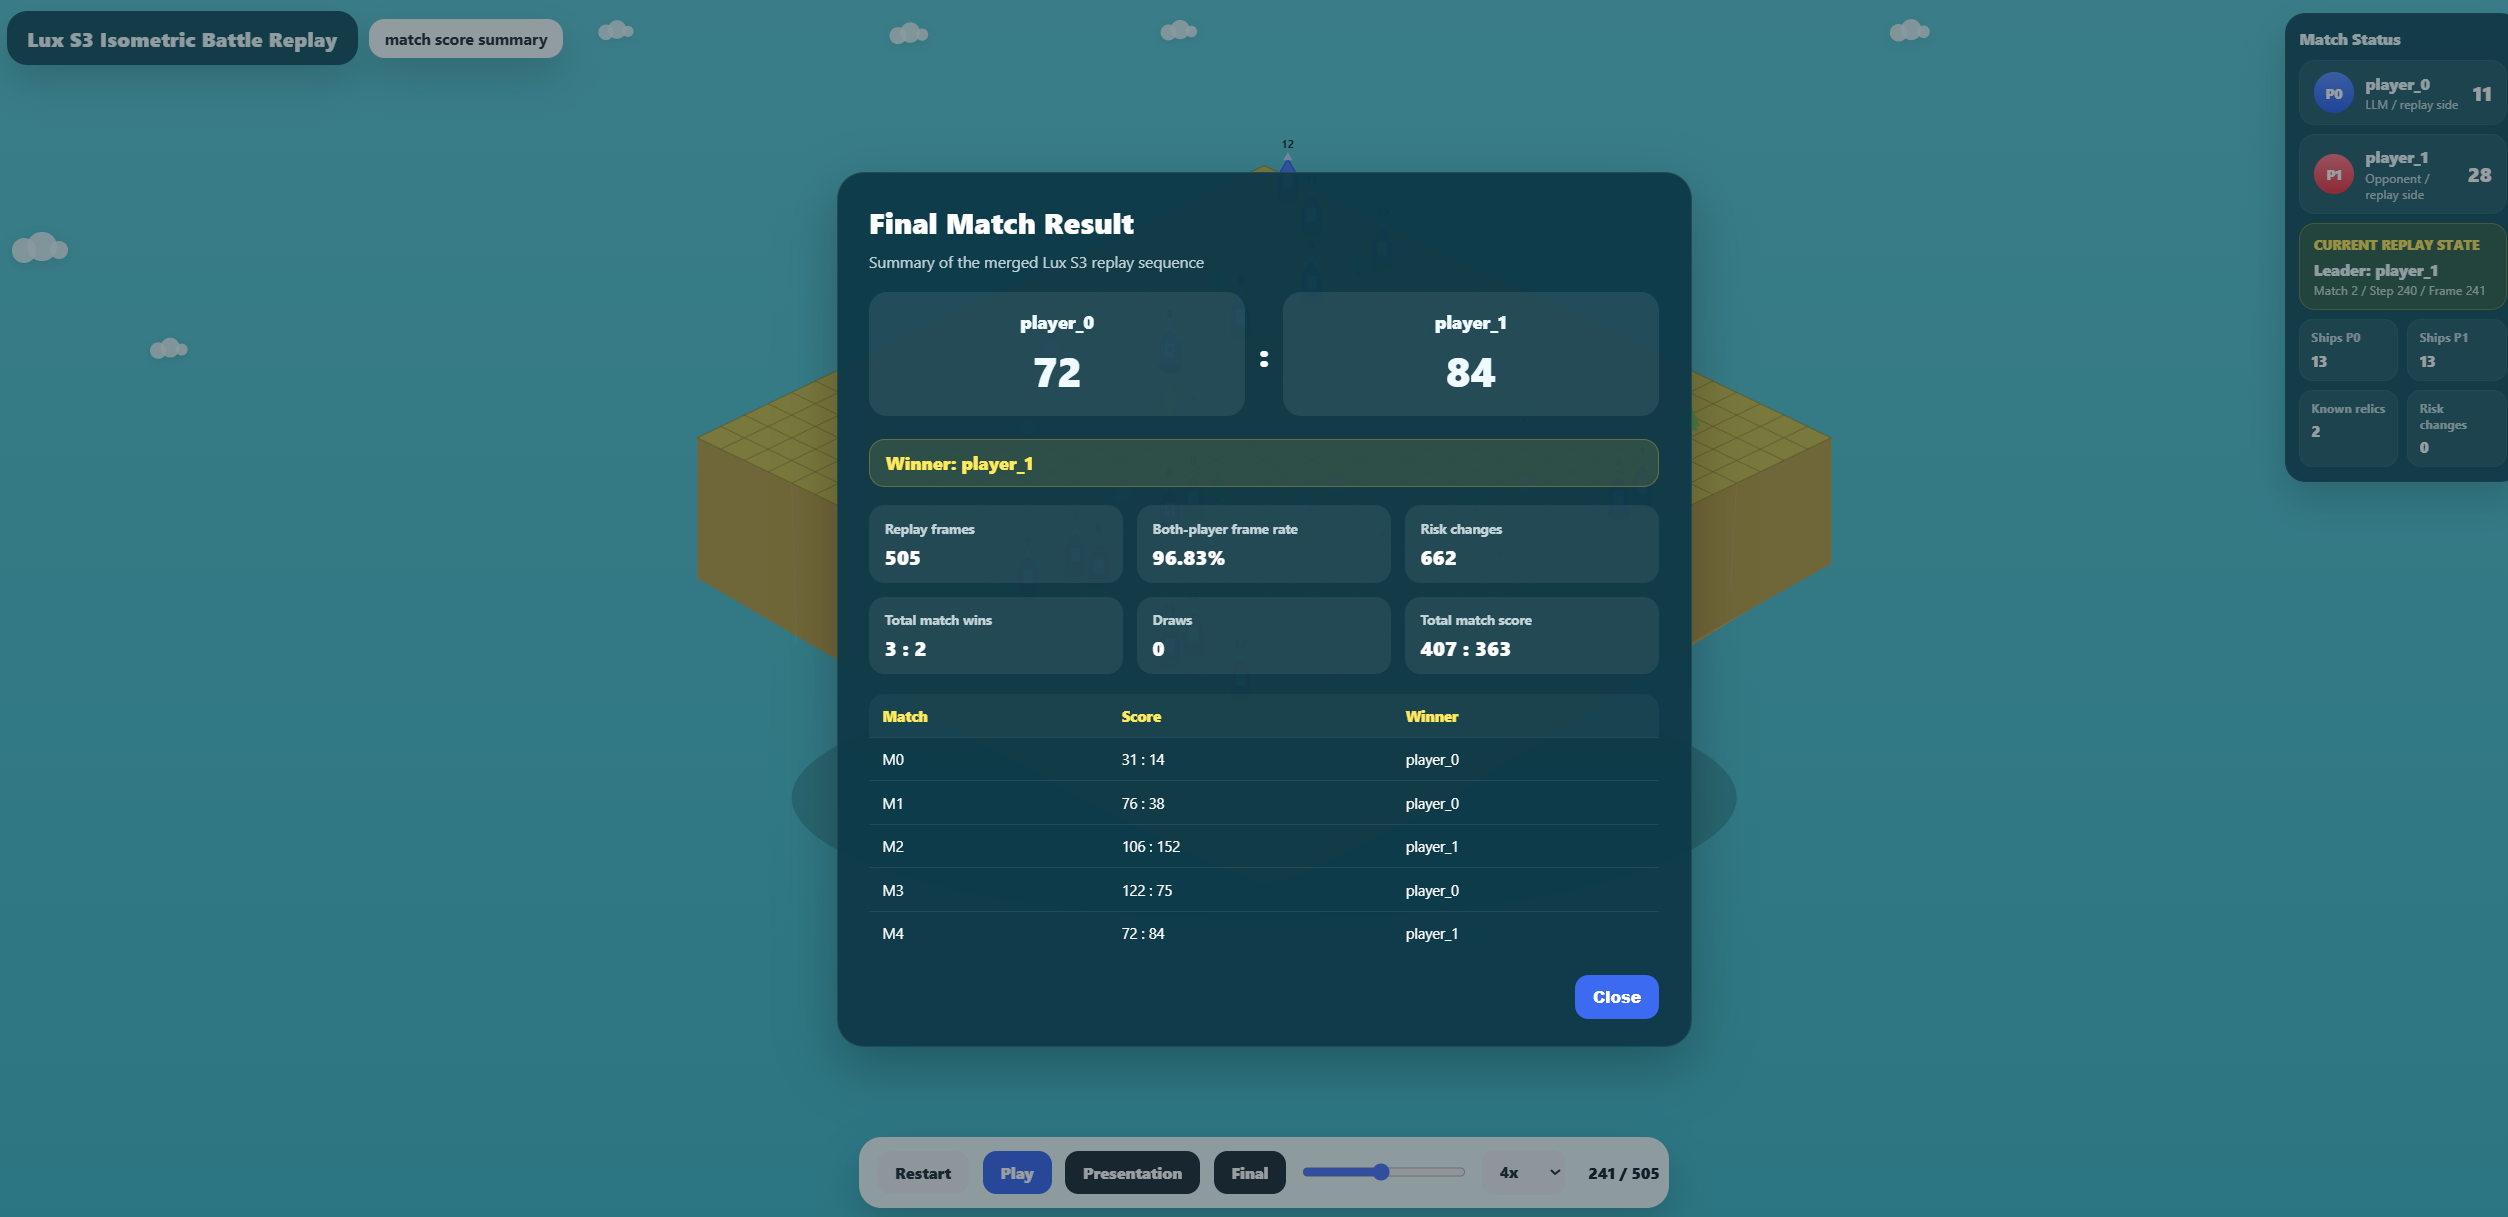
\includegraphics[width=\linewidth]{figures/figure_s3_final_result_overlay.png}
\caption{Final result overlay used by the replay viewer.}
\label{fig:final-overlay}
\end{figure}

\end{document}
